\subsection{Párovacia halda} 
\paragraph{Popis.}
Párovacia halda je ďalším druhom samoupravujúcej sa haldy. Opäť sa budeme pozerať na amortizovanú časovú zložitosť jej operácií.
Je to všeobecná halda, teda počet synov nie je obmedzený.
Základná procedúra, ktorú táto dátová štruktúra implementuje je spájanie (\emph{linking}) dvoch háld. Procedúra spočíva iba v tom, že sa halda s väčśím kľúčom v koreni napojí na tú s menším kľúčom. V našej implementácií sa nový vrchol napája vždy ako prvý syn.

\paragraph{Operácie.}
Operácia $\meld(i,j)$ využíva procedúru pre linking. Tiež $\ins(x)$, len prilinkuje novú jednoprvkovú haldu.
Operácia $\dec(v, \Delta)$ najprv zníži hodnotu vrcholu $v$, a keďže môže byť porušená podmienka pre haldu,
strom zakorenený vo vrchole $v$ sa odtrhne a prilinkuje ku zvyšku. Časové zložitosti pre všetky tieto operácie
sú $O(1)$. Najzaujímavejšie na párovacích haldách je \emph{deleteMin}. Po odstránení koreňa ostane les jeho detí.
Môžeme zvoliť niekoľko prístupov ako z detí vytvoríme nový strom.

Naivné riešenie hovorí, že si vyberieme jedno dieťa a ostatné k nemu prilinkujeme. Už na prvý pohľad vidíme,
že pri nesprávnom zvolení prvého dieťaťa môže byť časová zložitosť takéhoto algoritmu $O(n)$.

Ďalší, o niečo lepší nápad je deti najprv popárovať a prilinkovať. S výhliadkami do budúcnosti nám tento algoritmus dá 
amortizovanú časovú zložitosť $O(\sqrt{n})$.

\begin{figure}
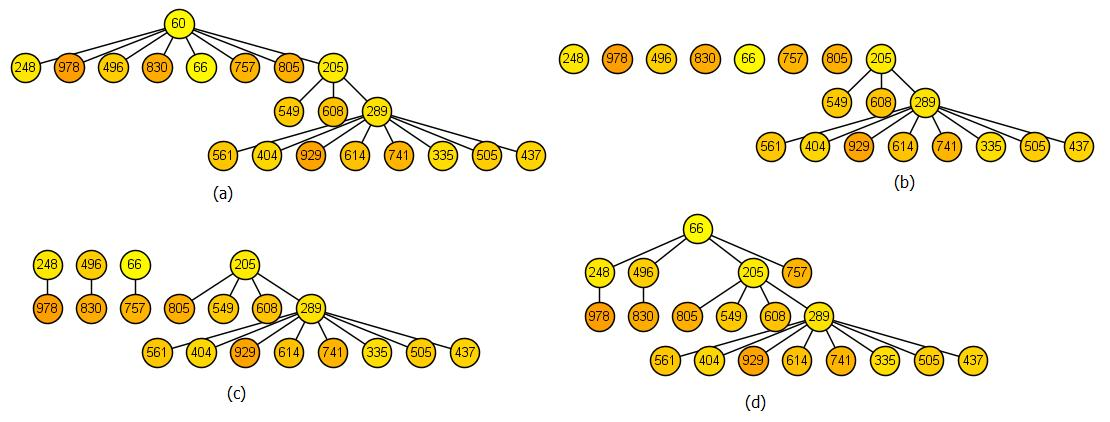
\includegraphics[width=\columnwidth]{obrazky/pairdel.png}
\caption{\emph{Vymazanie minima.} 
(a) pôvodná halda, (b) halda po vymazaní minima, (c) halda po párovaní, (d) halda po spájaní.} 
\label{img:pairdel} 
\end{figure}

Keď si dáme väčší pozor na to, ako deti párujeme, môžeme dosiahnnuť lepšie výsledky. Pokiaľ párujeme synov v poradí v akom boli prilinkovaní od najmladšieho a potom ich sprava doľava prilinkujeme, vieme dostať lepšie, avšak dosiaľ nedokázané výsledky.
Ostatné riešenia sme zatiaľ neimplementovali, preto len spomenieme, že sú popísané napríklad v \cite{pairing}.

Aby boli ale operácie efektívne, musíme zvoliť správnu reprezentáciu tejto dátovej štruktúry. V našom programe sme použili 
reprezentáciu pomocou binárneho stromu (\emph{binary tree represetation}), ktorú naprogramoval Viktor Tomkovič. V každom vrchole sa uchováva ľavý smerník na prvého syna, pravý smerník na nasledujúceho brata a ešte jeden smerník na rodiča.

\paragraph{Vizualizácia.}
Aby sa dala vizualizácia \emph{deleteMin} lepšie previesť, minimum, teda koreň haldy ostáva súčasťou haldy až do konca operácie, ale je zneviditeľnený. Navonok teda vyzerá, že po odstránení minima ostal les synov, ale v skutočnosti je to stále jedna halda. Týmto využijeme už naprogramované rozloženie vrcholov a nemusíme zavádzať nové pole pre synov.